Para la pantalla de inicio, se solicitaba que al ingresar, el usuario pudiera observar un pequeño resumen de los dispositivos que estaban siendo monitoreados en ese momento, dicho resumen debía contener los siguientes puntos:
\begin{itemize}
\item Número de dispositivos monitorizados.
\item Status de conexión de cada dispositivos.
\item El número de interfaces de red que estaban disponibles de cada dispositivo.
\item Status de cada interfaz de dichos dispositivos.
\end{itemize}

De esta forma, la pantalla inicial de nuestro administrador es como la siguiente (figura \ref{image:ejecucionP}), en la que se separa con pequeños titulares cada uno de los puntos solicitados y en donde se observan los datos de cada dispositivo que estaba siendo monitoreado en ese momento.
\FloatBarrier
\begin{figure}[htbp!]
		\centering
	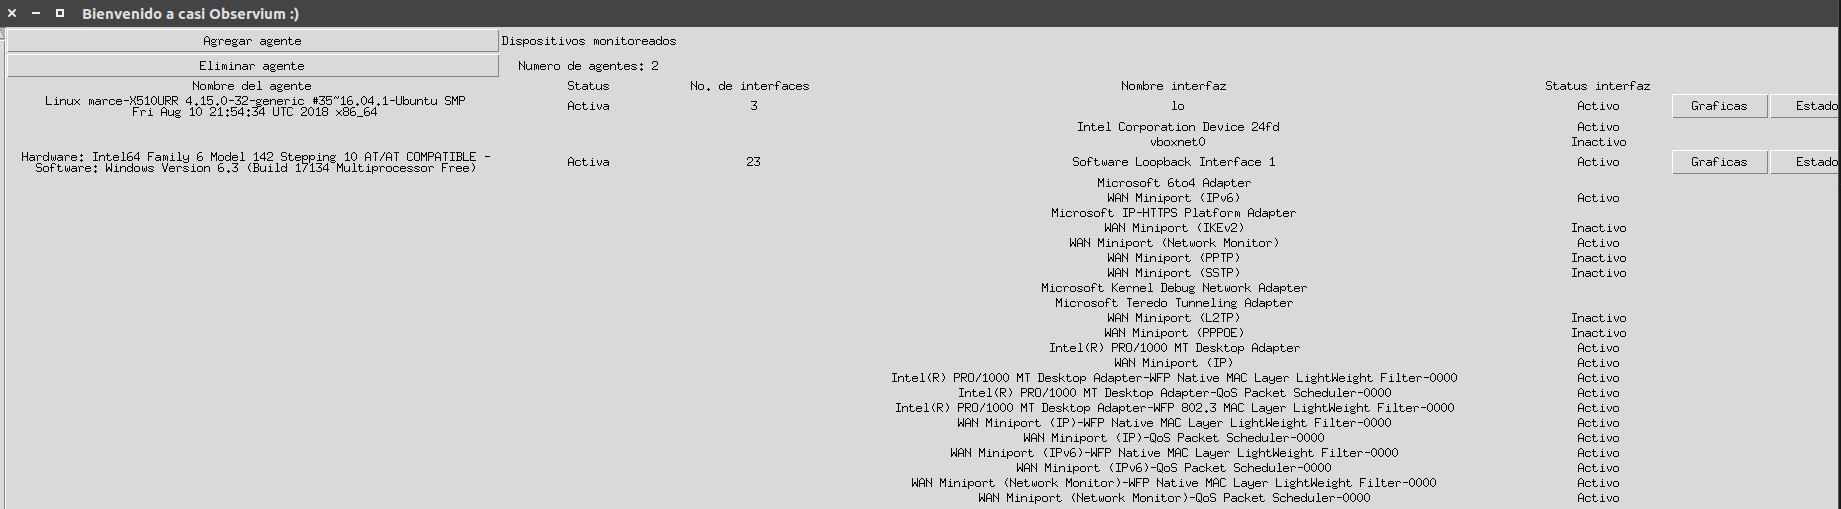
\includegraphics[width=1.1 \textwidth]{images/ejecucionP}
		\caption{Pantalla principal.}		\label{image:ejecucionP}
\end{figure}
\FloatBarrier

A continuación explicaré el código más importante de esta sección.
\\ \par
Primero se ejecuta el método llamado getHostInfo como se muestra en la figura  \ref{image:principal0}
\FloatBarrier
\begin{figure}[htbp!]
		\centering
	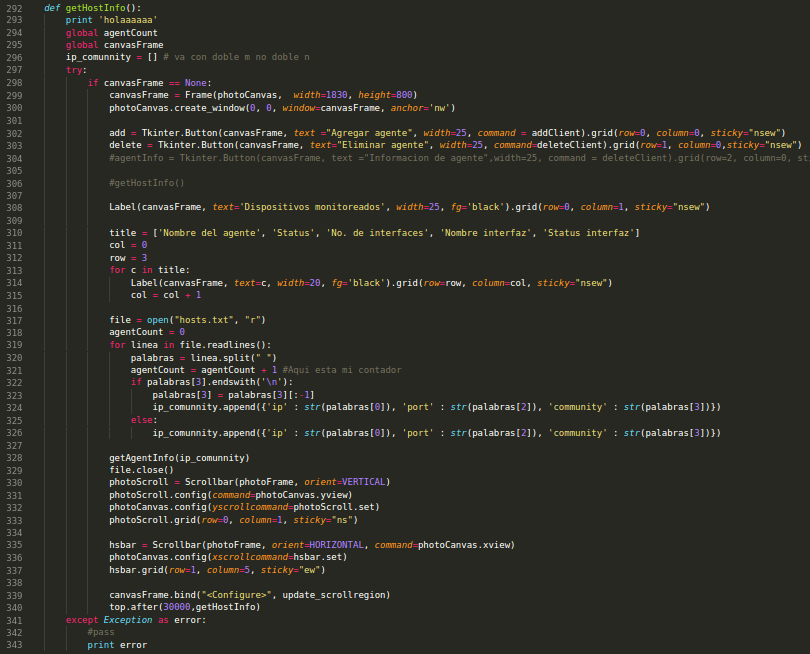
\includegraphics[width=.75 \textwidth]{images/principal0}
		\caption{Método getHostInfo.}		\label{image:principal0}
\end{figure}
\FloatBarrier

Dentro del cuál se observan las siguientes líneas de la figura \ref{image:principal1} en las que se abre nuestro archivo de hosts.txt en el cual se almacena la información de cada agente. Se consulta dicho archivo, se obtiene la información línea por línea de cada agente y se almacenan esos datos en un arreglo que será consultado posteriormente. 
\FloatBarrier
\begin{figure}[htbp!]
		\centering
	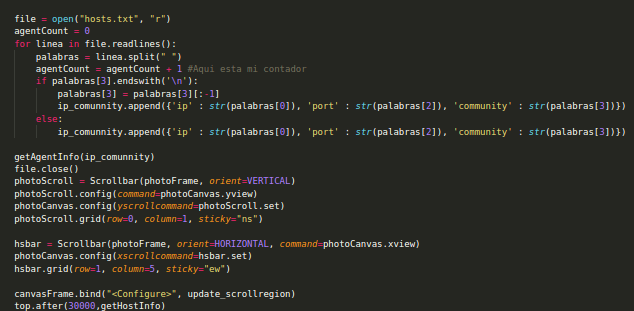
\includegraphics[width=.9 \textwidth]{images/principal1}
		\caption{Método getHostInfo, líneas importantes.}		\label{image:principal1}
\end{figure}
\FloatBarrier

Como se puede observar en la figura anterior, en unas líneas más abajo se manda a llamar a nuestro siguiente método a mostrar, el método getAgentInfo mostrado a continuación en la figura \ref{image:principal2}.
\FloatBarrier
\begin{figure}[htbp!]
		\centering
	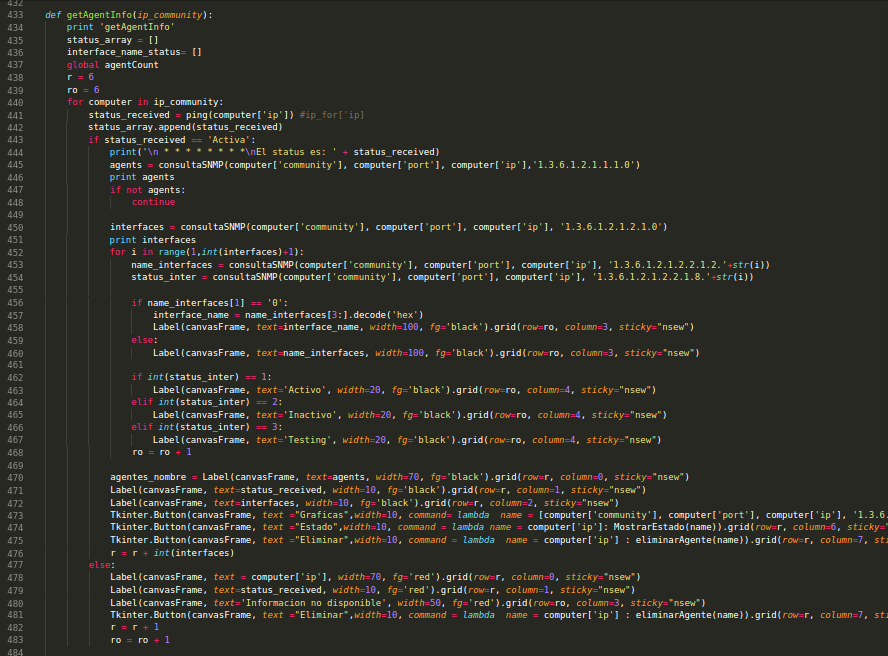
\includegraphics[width=.75 \textwidth]{images/principal2}
		\caption{Método getAgentInfo.}		\label{image:principal2}
\end{figure}
\FloatBarrier

Al cual, nuevamente mostraremos solo las líneas principales en la siguiente figura \ref{image:principal3} en donde se realiza una actividad muy importante, se envían los datos de cada uno de los agentes con un OID en específico para obtener su información y posteriormente plasmarla en sus respectivos labels.
\FloatBarrier
\begin{figure}[htbp!]
		\centering
	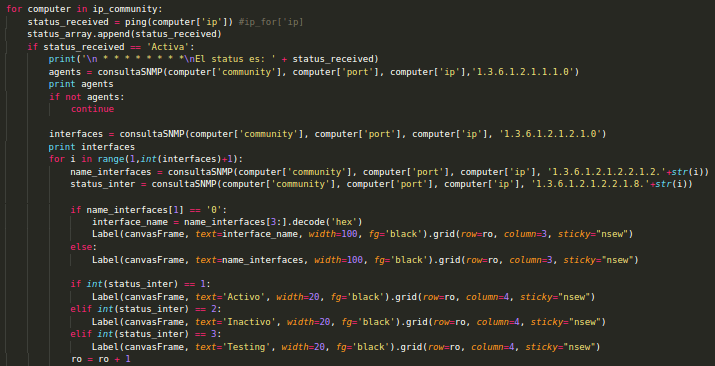
\includegraphics[width=.95 \textwidth]{images/principal3}
		\caption{Método getAgentInfo, líneas importantes.}		\label{image:principal3}
\end{figure}
\FloatBarrier

Por último, es importante mostrar 2 métodos igualmente importantes, uno es el método ping mostrado en la figura \ref{image:ping} con el cual se verifica si la ip está activa o no y en caso de no estarlo, no buscar su información en la MIB.
\FloatBarrier
\begin{figure}[htbp!]
		\centering
	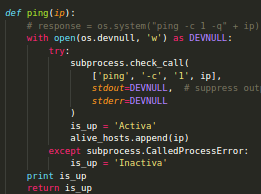
\includegraphics[width=.4 \textwidth]{images/ping_1}
		\caption{Método ping.}		\label{image:ping}
\end{figure}
\FloatBarrier
Por otro lado, el otro método a mostrar es el de la figura \ref{image:mib} mediante el cual, se ejecuta la instrucción snmpget y se obtiene la información solicitada.
\FloatBarrier
\begin{figure}[htbp!]
		\centering
	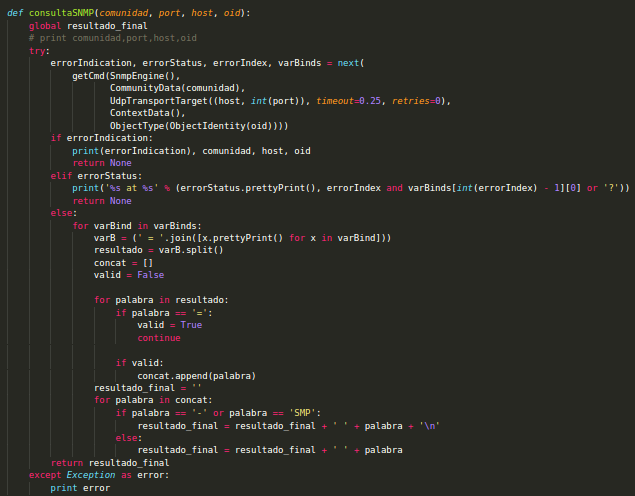
\includegraphics[width=.8 \textwidth]{images/mib}
		\caption{Método consultaSNMP.}		\label{image:mib}
\end{figure}
\FloatBarrier